\documentclass[UTF8, 11pt, fontset=none]{ctexart}
\setCJKmainfont{Source Han Serif SC}
\usepackage[T1]{fontenc}

\setCJKmonofont{Source Han Mono SC}
\usepackage{underscore}

\pagestyle{plain}
\ctexset{section/format=\Large\bfseries}
\usepackage[a4paper, hmargin=1.5cm, vmargin=1.9cm]{geometry}
\setlength{\parskip}{0.5em}
\usepackage{enumitem}
\setlist{topsep=0pt,itemsep=-4pt}

\usepackage{amsmath}
\usepackage{amssymb}
\usepackage[separate-uncertainty=true]{siunitx}[=v2]

\usepackage{multirow}
\usepackage{diagbox}

\usepackage[pdfusetitle, colorlinks, urlcolor=blue, linkcolor=black]{hyperref}
\usepackage{graphicx}
\usepackage{float}
\usepackage{cleveref}
\crefname{figure}{图}{图}
\crefname{table}{表}{表}
\crefname{page}{页}{页}
\crefname{section}{节}{节}

\usepackage[normalem]{ulem}

\begin{document}

\title{数字逻辑设计 12 组(Chrome 小恐龙)实验报告}
\author{致理-信计 11 \hspace{2pt} 游宇凡 \hspace{12pt} 计14 \hspace{2pt} 王博文}
\maketitle

\section{项目介绍}

《恐龙游戏》(英语:Dinosaur Game)是一款内置于 Google Chrome 的网页游戏,会在用户断网时自动出现,也可以通过访问 \texttt{chrome://dino} 来游玩。玩家在横向滚动栏形式的恐龙游戏中,操控一只像素风格的小暴龙跳跃、下蹲以避开障碍物并获取分数。

\begin{figure}[H]
    \centering
    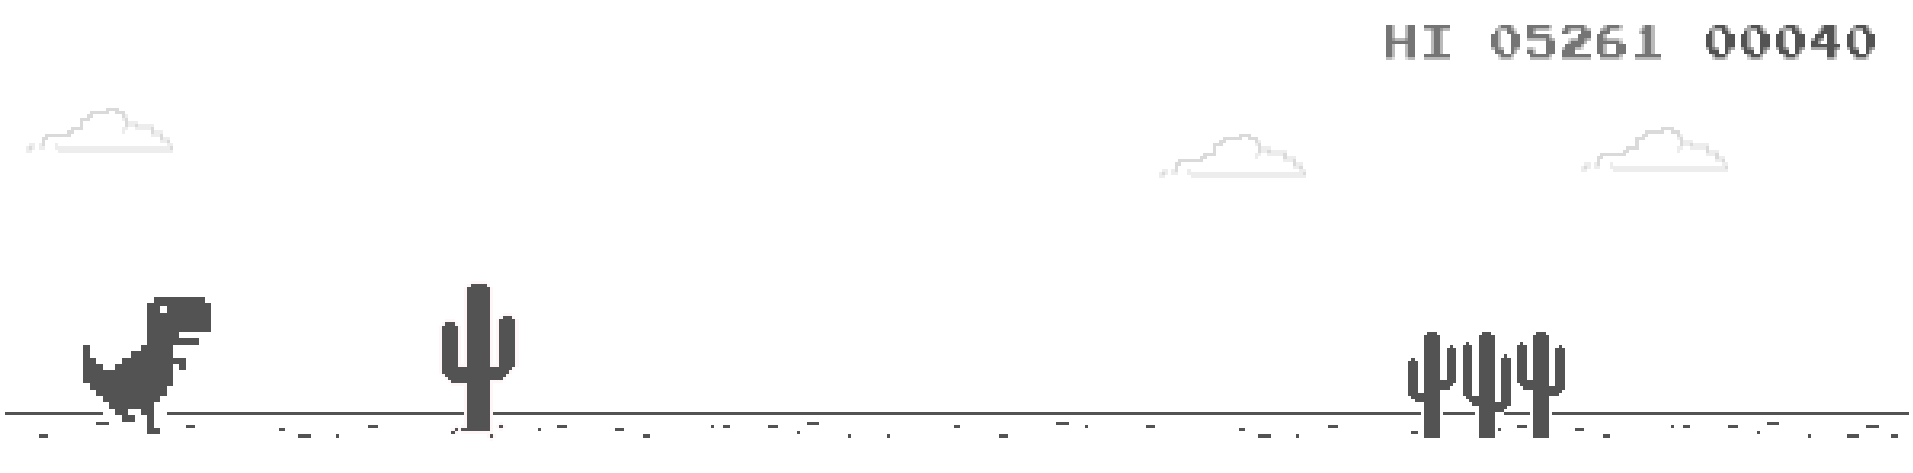
\includegraphics[width=\textwidth]{images/cover.png}
    \caption{Chrome 恐龙游戏截图}
    \label{cover}
\end{figure}

我们使用 FPGA 复刻这一游戏,支持按键和传感器两种输入方式,并使用 VGA 输出。使用传感器时,需要玩家将传感器绑在大腿上,传感器将检测玩家跳跃和下蹲的动作,在增加趣味性的同时,还能起到一定的健身作用。\scriptsize\sout{(测试的时候跳得确实很累)}\normalsize

\section{总体设计}

\subsection{模块总体划分和分工}

总体设计分为传感器模块、画面输出模块和游戏逻辑模块。

我们的分工非常简明,由游宇凡同学负责传感器(外设组装调试以及代码编写)和画面输出,由王博文同学负责游戏逻辑。两位同学所负责模块之间的接口也非常简单,只有蹲下、起跳的信号,画面上每个元素的坐标信息,控制昼夜转换的信号,以及画面刷新信号、时钟信号等,这大大降低了我们的沟通成本。

\subsection{文件说明}

\begin{table}[H]
    \centering
    \caption{文件说明}
    \vspace{1em}
    \small
    \begin{tabular}{|c|c|c|c|}
        \hline
        目录 & 文件名 & 描述 & 主要完成者 \\
        \hline
        \multirow{20}*{\texttt{src}}
            & \texttt{async_receiver.sv} & 接收 UART 数据 & 游宇凡 \\ \cline{2-4}
            & \texttt{cloud.sv} & 云朵 & 王博文 \\ \cline{2-4}
            & \texttt{distance_meter.sv} & 记分板 & 王博文 \\ \cline{2-4}
            & \texttt{dpy_scan.v} & 实验板上的数码管显示 & 助教(即提供的代码模板) \\ \cline{2-4}
            & \texttt{horizon.sv} & 管理动态场景元素 & 王博文 \\ \cline{2-4}
            & \texttt{horizon_line.sv} & 地面 & 王博文 \\ \cline{2-4}
            & \texttt{mod_top.sv} & 顶层模块 & 游宇凡、王博文、助教 \\ \cline{2-4}
            & \texttt{motion_detector.sv} & 由传感器数据判断运动状态 & 游宇凡 \\ \cline{2-4}
            & \texttt{night.sv} & 星空和月亮 & 王博文 \\ \cline{2-4}
            & \texttt{obstacle.sv} & 障碍物 & 王博文 \\ \cline{2-4}
            & \texttt{painter.sv} & 逐个绘制背景和画面元素 & 游宇凡、王博文 \\ \cline{2-4}
            & \texttt{paint_background.sv} & 绘制画面空白背景 & 游宇凡 \\ \cline{2-4}
            & \texttt{paint_element.sv} & 基于 sprite 图绘制单个画面元素 & 游宇凡 \\ \cline{2-4}
            & \texttt{palette.sv} & 由颜色编号以及昼夜转换获取 RGB 值 & 游宇凡 \\ \cline{2-4}
            & \texttt{resetter.sv} & 启动时自动复位,之后按按钮复位 & 游宇凡、王博文 \\ \cline{2-4}
            & \texttt{runner.sv} & 游戏逻辑控制模块 & 王博文 \\ \cline{2-4}
            & \texttt{sensor.sv} & 解析传感器数据 & 游宇凡 \\ \cline{2-4}
            & \texttt{spike_filter.sv} & 信号消抖(用于 UART) & 游宇凡 \\ \cline{2-4}
            & \texttt{synchronizer.sv} & 异步信号同步化(用于 UART) & 游宇凡 \\ \cline{2-4}
            & \texttt{trex.sv} & 小恐龙 & 王博文 \\ \cline{2-4}
            & \texttt{vga.sv} & 显存 \& VGA 输出 & 游宇凡、助教 \\ \hline
        \multirow{7}*{\texttt{src/sim}}
            & \texttt{async_receiver_sim.sv} & \multirow{7}*{相应模块的仿真测试} & 游宇凡 \\ \cline{2-2} \cline{4-4}
            & \texttt{distance_meter_sim.sv} & & 王博文 \\ \cline{2-2} \cline{4-4}
            & \texttt{horizon_sim.sv} & & 王博文 \\ \cline{2-2} \cline{4-4}
            & \texttt{obstacle_sim.sv} & & 王博文 \\ \cline{2-2} \cline{4-4}
            & \texttt{runner_sim.sv} & & 王博文 \\ \cline{2-2} \cline{4-4}
            & \texttt{sensor_sim.sv} & & 游宇凡 \\ \cline{2-2} \cline{4-4}
            & \texttt{trex_sim.sv} & & 王博文 \\ \hline
        \multirow{4}*{\texttt{src/util}}
            & \texttt{collision.sv} & 碰撞检测函数 & 王博文 \\ \cline{2-4}
            & \texttt{lfsr.v} & 线性反馈移位寄存器 & Alex Forencich \\ \cline{2-4}
            & \texttt{lfsr_prng.sv} & 基于 LFSR 的伪随机数生成器 & Alex Forencich \\ \cline{2-4}
            & \texttt{util_func.sv} & 全局辅助函数 & 王博文 \\ \hline
        \texttt{tools} & \texttt{image-to-mif.py} & 将图片转换为 MIF 文件(3 bit 字宽) & 游宇凡 \\ \hline
        \multirow{3}*{\texttt{assets}}
            & \texttt{sprite.xcf} & \multirow{2}*{基于原版 sprite 图进行了一些修改} & Chromium、游宇凡 \\ \cline{2-2} \cline{4-4}
            & \texttt{sprite.png} & & 由 GIMP 生成 \\ \cline{2-4}
            & \texttt{sprite.mif} & 存于 ROM 中的 sprite 图 & 由 \texttt{image-to-mif.py} 生成 \\ \hline
    \end{tabular}
    \normalsize
    \label{file-description}
\end{table}

\section{模块设计}

整体模块设计如\cref{modules} 所示。

\begin{figure}[H]
    \centering
    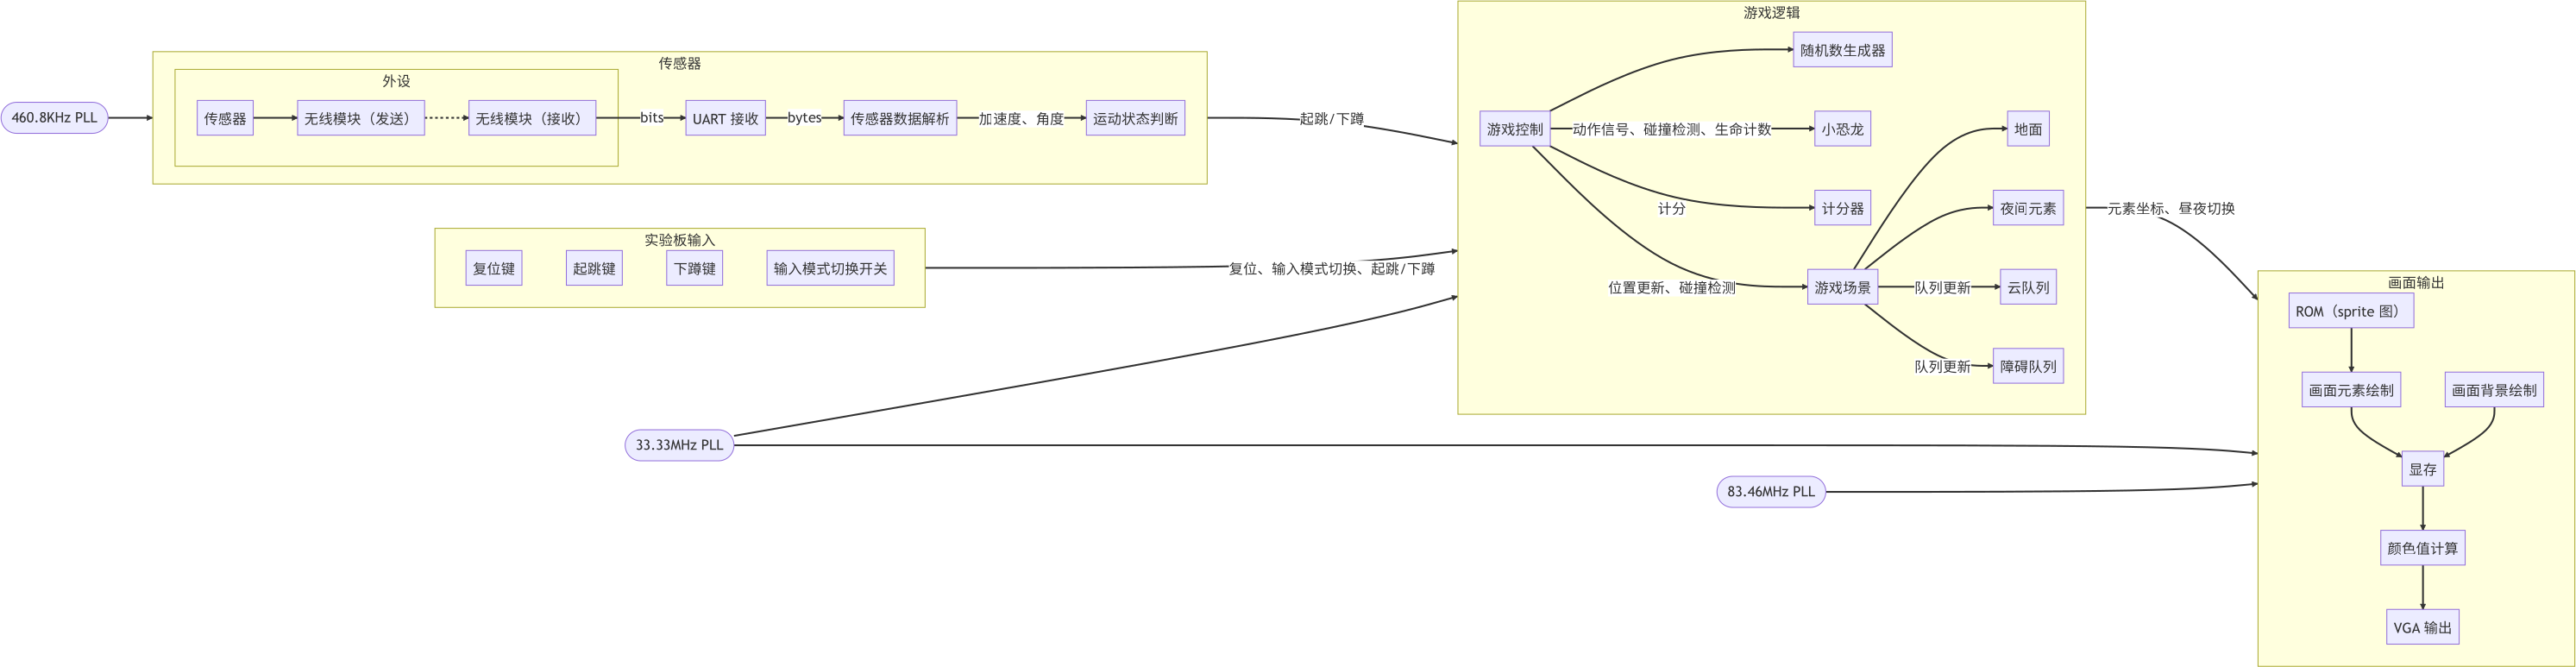
\includegraphics[width=\textwidth]{images/modules.png}
    \caption{整体模块划分示意图}
    \label{modules}
\end{figure}

\subsection{传感器模块}

\subsubsection{外设组装}

采用一个维特智能九轴加速度计陀螺仪磁场姿态角度传感器模块 JY901S 测量玩家的运动数据,以及一对 HC-12 无线模块来向实验板传输数据。

在组装外设之前,先使用 USB 转 TTL 模块依次将传感器和两个无线模块连接到电脑上,并使用配套的软件将它们的波特率都设为 \SI{57600}{bps}。各个模块的波特率默认均为 \SI{9600}{bps},调高波特率可以允许更高的数据测量频率,进而提升运动状态检测的准确性。

将天线焊接在无线模块上,传感器一侧的各个元件之间直接焊接相连(TX 与 RX 相连),固定在面包板上,由充电宝和 USB 转 TTL 模块进行供电,整体放在为 Switch 健身环设计的绑腿中,如\cref{sensor} 所示。

因为无线模块的 VCC、GND 引脚以及 Pmod 接口的供电引脚刚好都位于最外侧,实验板一侧的无线模块直接插在 Pmod 1 接口上的 $2 \sim 6$ 引脚。

\begin{figure}[ht]
    \centering
    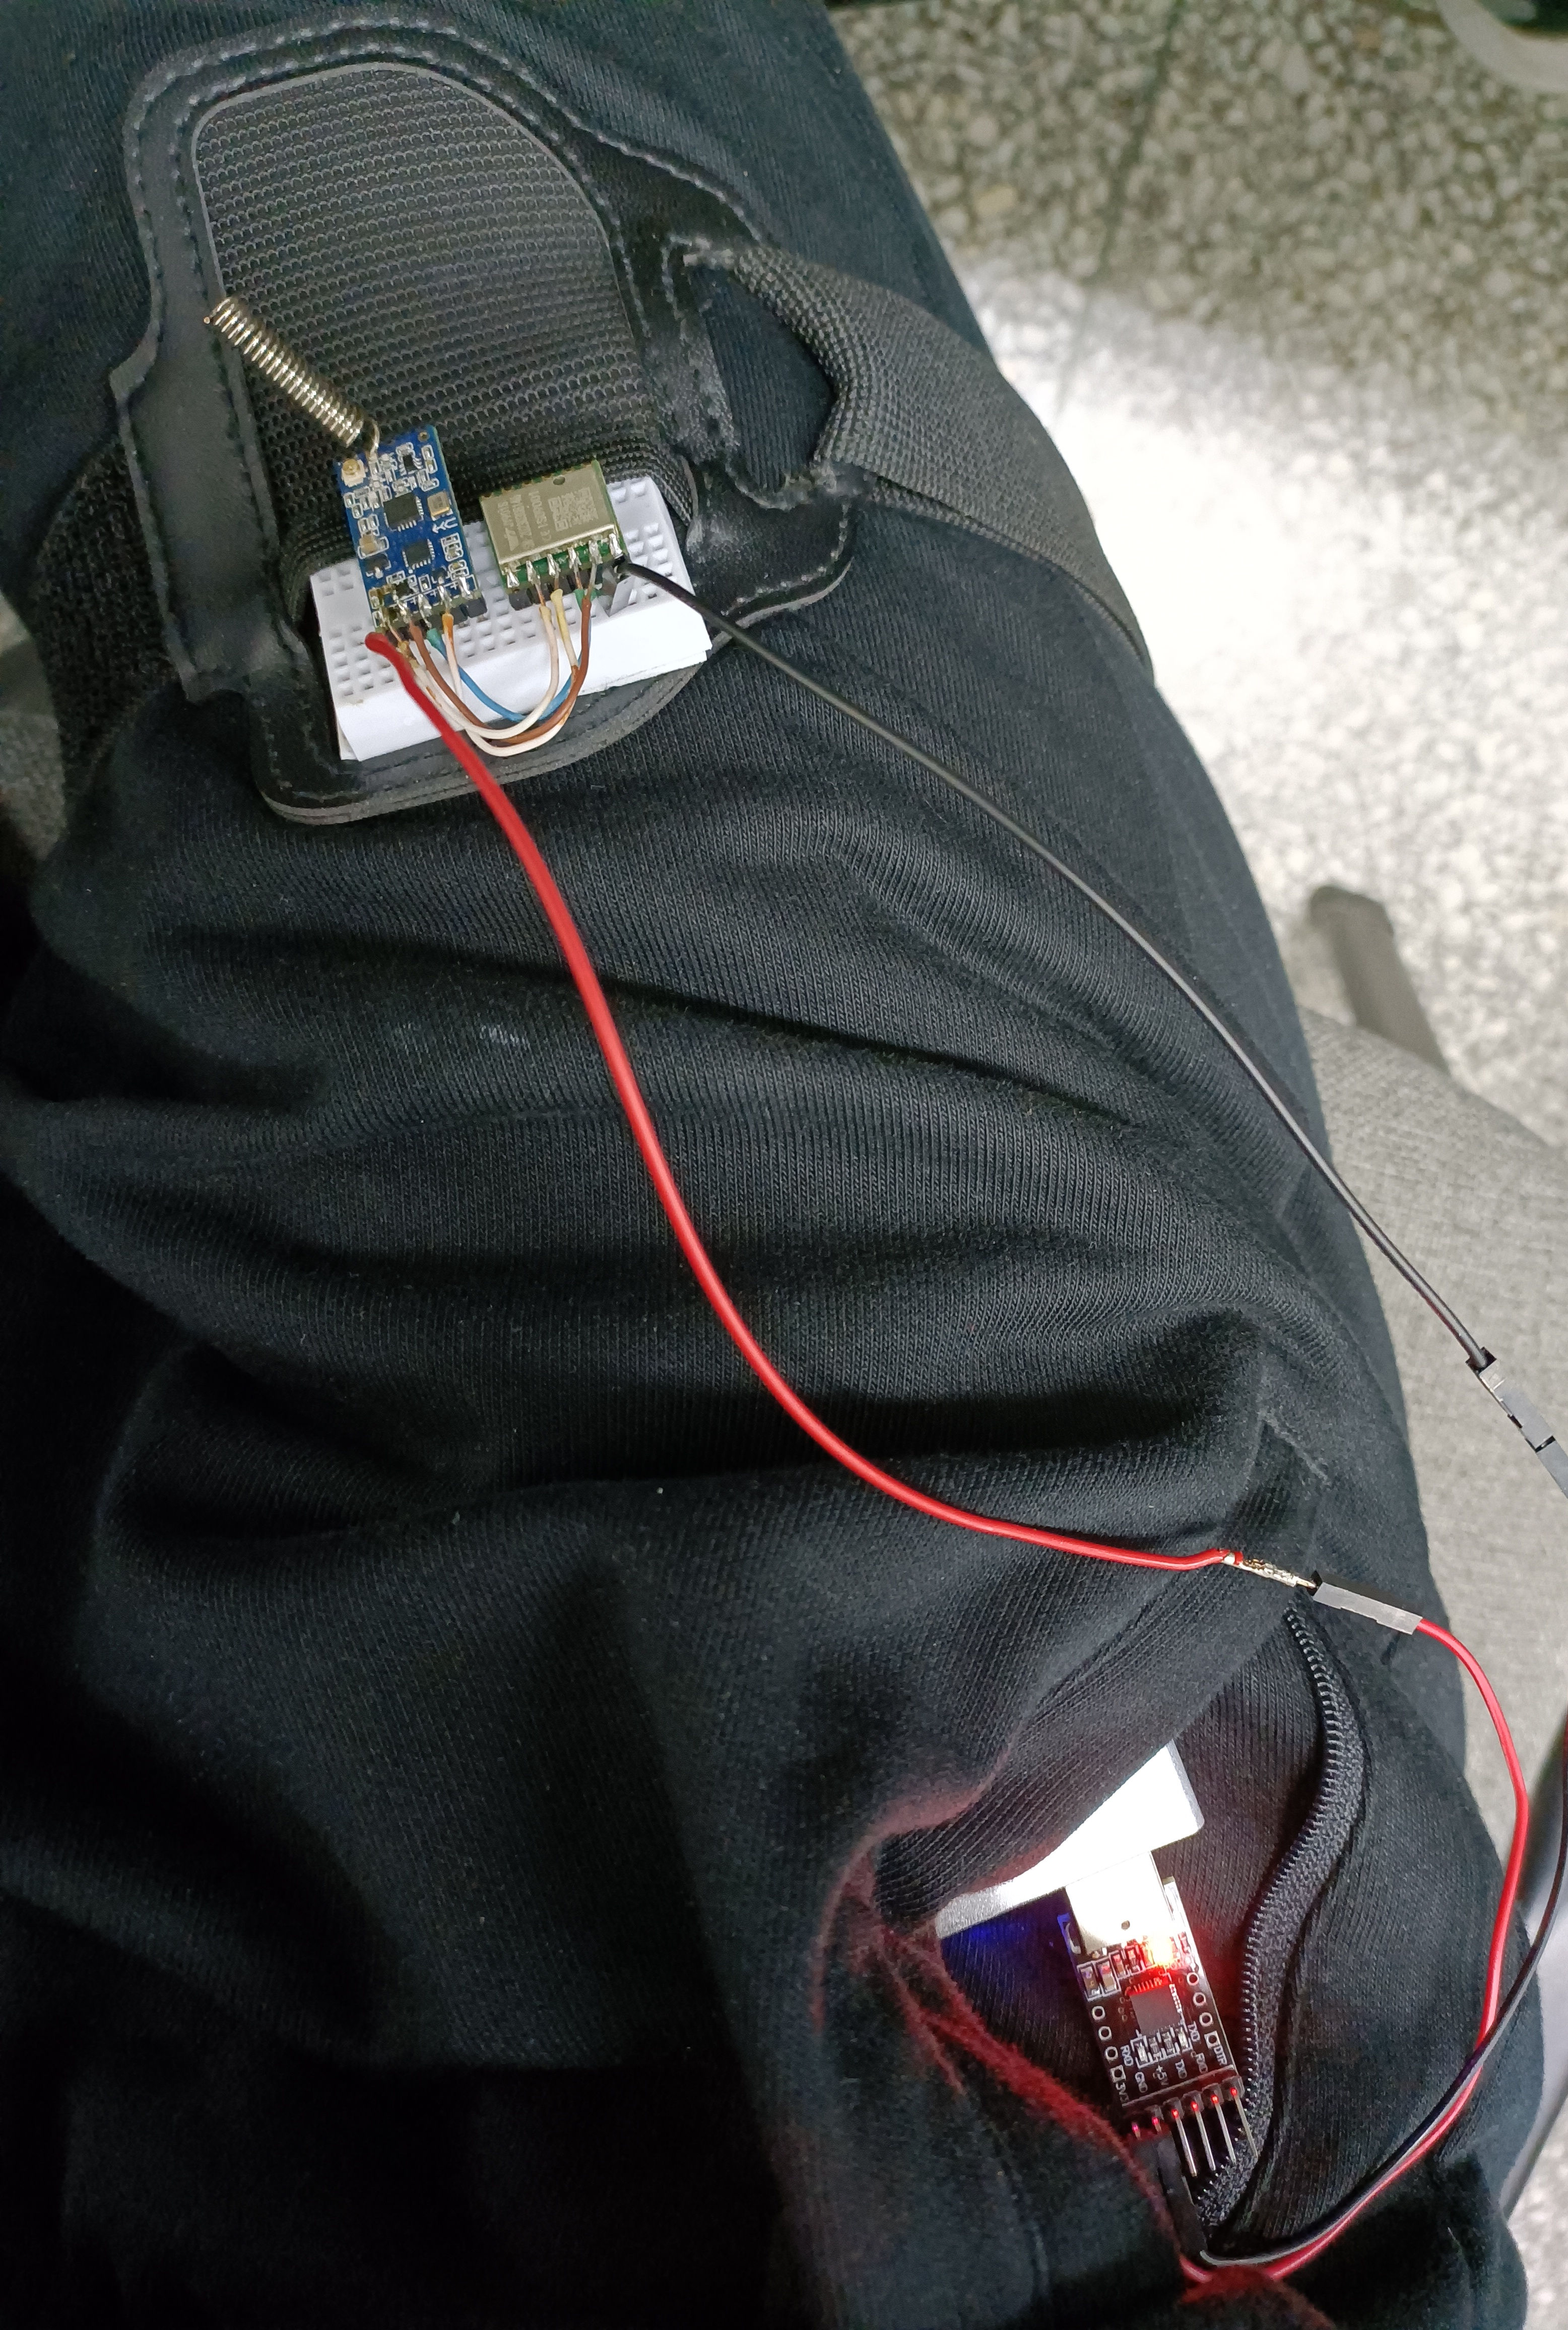
\includegraphics[width=0.5\textwidth]{images/sensor.jpg}
    \caption{外设实拍图}
    \label{sensor}
\end{figure}

\subsubsection{UART 数据接收}

参考 \href{https://www.fpga4fun.com/SerialInterface.html}{fpga4fun - Serial interface} 编写了 UART 数据接收。在 UART 协议中,以预先设定的波特率为频率传输 bit,而以 byte 为单位传输数据。传输每个 byte 时,先以 0 表示开始,然后由小端序的 8 个 bit 表示数据,之后保持 1 直到下一个 bit,如\cref{uart} 所示。具体接收流程为:

\begin{enumerate}
    \item 使用 PLL 提供频率为波特率 8 倍的时钟来进行过采样
    \item 将从 RX 接收到的信号同步到时钟,并消除毛刺信号
    \item 使用状态机依次完成一个 byte 传输过程中的每一步:
        \begin{enumerate}
            \item 开始接收后,使用一个 $0 \sim 7$ 的计数器,每数到 3(此时大约是一个 bit 的中点)读取下一个 bit
            \item 在接收到 0 时开始整个接收过程,即状态机变为开始接收的状态,计数器置 0
            \item 在过程中,使用一个移位寄存器来读取这个 byte
            \item 读完这个 byte 后,输出表示 byte 读取完毕的信号(即只有这个信号为 1 时,UART 读取模块对外输出的 byte 值才是有效的),然后回到等待开始的状态
        \end{enumerate}
\end{enumerate}

\begin{figure}[H]
    \centering
    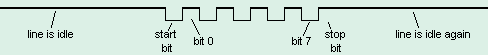
\includegraphics[width=\textwidth]{images/uart.png}
    \vspace{-16pt}
    \caption{UART 协议示意图(来自 \url{https://www.fpga4fun.com/SerialInterface1.html})}
    \label{uart}
\end{figure}

\subsubsection{传感器数据解析}

参考 \href{https://wit-motion.yuque.com/wumwnr/ltst03/vl3tpy}{WIT 私有协议} 使用状态机逐字节接受数据并解析:

\begin{enumerate}
    \item 接收到协议头 \texttt{0x55} 后开始整个读取过程
    \item 读取包括协议头在内的前 10 个 byte 时,将每个 byte 加在一起计算 sumcrc
    \item 第 2 个 byte 表示消息类型,读取时记录下来
    \item 后面 8 个 byte 每两个 byte 表示一个数据的低位和高位,根据消息类型,读到需要的数据时记录下来
    \item 第 11 个 byte 是 sumcrc,若读取到的 sumcrc 和计算得到的相同这次读取才有效,根据消息类型,使用记录下的数据更新模块对外的输出
\end{enumerate}

\subsubsection{动作判断}

采用简单的阈值判断来检测玩家起跳/下蹲的动作:与水平方向夹角小于 \SI{56.25}{\degree} 则判断为下蹲,竖直方向含 $g$ 的加速度大于 $-0.25 g$(向下为正,静止时理论上是 $-1g$)则判断为起跳。

\subsection{画面输出模块}

图像的绘制基于原版恐龙游戏使用的 \href{https://github.com/chromium/chromium/blob/3b31f1cbd28e0a1199defe6f6b37001cef4c4790/components/neterror/resources/images/default_200_percent/offline/200-offline-sprite.png}{sprite 图},采用 \href{http://tinyvga.com/vga-timing/1280x800@60Hz}{1280$\times$800 @ 60Hz} 的分辨率,其中 1280$\times$300 的部分是实际游戏画面,和原版画面大小大致相同,剩下的部分是空白。

\subsubsection{显存 \& VGA 输出}

采用双显存机制,将片内 RAM 的一半用于写入,一半用于读取,每帧对两块显存进行交换。通过 ring buffer 修复读取缓存产生的延时导致的像素偏移。显存采用 \SI{33.33}{\mega\hertz} 的写入时钟和 VGA 所需的 \SI{83.46}{\mega\hertz} 读取时钟。VGA 模块提供一个画面刷新信号输出,用来告诉游戏逻辑模块需要更新画面。

VGA 模块还接受黑夜程度作为输入以实现昼夜转换,为了支持渐变还需要得到过程中的颜色值,如果直接进行乘法运算会有较大的延时,难以在 VGA 的高频时钟下完成计算,所以实际采用的方案是在编译时就计算出所有可能的颜色值(具体实现为使用 $0 \sim 63$ 作为 \texttt{parameter} 分别进行实例化),根据黑夜程度进行选择。

\subsubsection{sprite 图编辑}

原版 sprite 共有 17 种颜色,通过 GIMP 压缩至只有 8 种颜色,使得 ROM 和显存中每个像素只占据 3 个 bit,并且裁剪掉未使用的部分,从而可以放进 FPGA 的内置存储资源(共使用 $2442 \times 130 \times 3 + 2 \times 1280 \times 300 \times 3 \approx \SI{3.26}{\mega b}$ 存储资源)。

除了压缩,还添加了若干元素,包括生命值的图标,以及数字的浅色版本(用于最高分的显示,原版 sprite 中没有浅色的数字,而是通过调整透明度实现的浅色)。

\subsubsection{元素绘制}

sprite 图转为 MIF 文件存在片内 ROM 中。元素绘制模块接受 sprite 坐标、画面绘制坐标、元素宽高作为参数,通过状态机依次绘制空白背景和每个元素,绘制每个元素时通过状态机枚举坐标进行绘制,从 ROM 中读取每个像素,通过 ring buffer 修复因读取 ROM 产生的偏移。

\subsection{游戏逻辑模块}

\subsubsection{游戏控制}

游戏控制模块接受按键信号和传感器信号,进行游戏内部计时器的更新并触发各个游戏元素的状态更新,同时输出游戏元素的坐标信息。
这一模块的源代码主要位于 \texttt{runner.sv} 中。

具体说来,游戏控制模块维护了一个状态机,包含等待 (Waiting)、运行 (Running)、结束 (Crashed) 和重启 (Restarting) 四个状态。
\begin{description}
    \item[等待] 这一状态下,游戏控制模块会等待玩家按下开始游戏的按键,或者等待传感器检测到玩家的跳跃动作,之后转入运行状态。
    \item[运行] 这一状态是游戏的正常运行状态。在这一状态下,碰撞检测、昼夜切换等功能将正常运行,同时各个游戏元素也将正常更新运动。
    \item[结束] 当碰撞检测模块检测到小恐龙与障碍发生碰撞时,将会扣除一条生命值。如果生命值耗尽,将会转入结束状态,此时所有模块将不再更新,展示游戏结束画面并记录最高分。
    \item[重启] 若玩家在结束状态下进行一次跳跃,将会重启游戏,此时除了记录的最高分外将会重置,小恐龙将会回到起点,同时生命值也会恢复。之后,控制模块重新转入等待状态。此外,为了避免使用传感器时玩家意外跳跃导致游戏重启,我们还在重启状态下增加了一个计时器,只有在游戏结束一小段时间后玩家才能重启游戏。
\end{description}

为了更好地同步画面输出与游戏更新,我们让画面输出模块输出了一个更新完成 (\texttt{painter_finished}) 信号。
画面更新完成的同时,游戏控制模块就将进行下一帧游戏逻辑的执行。

此外,游戏控制模块还负责维护当前的游戏速度。这一速度在逻辑上是小恐龙的跑动速度,在实现上它体现为场景向左的运动速度。

\subsubsection{随机数生成}

我们发现如果所有障碍物的间隔和类型都是固定的,游玩起来将非常枯燥,因此我们引入了随机因素,让玩家必须根据动态生成的障碍物来进行快速反应,同时也让每一局游戏都有所不同。

为了做到这一点,我们采用了 Alex Forencich 编写的 Verilog LFSR 伪随机数生成器 (\texttt{util/lfsr.sv}, \texttt{util/lfsr_prng.sv}) 进行伪随机数的生成。
玩家可以采用实验板上的拨码开关提供随机数种子的一部分,同时我们也采用了当前的系统时间作为另一部分随机数种子。
具体地,我们在玩家开始游戏的一瞬间采样游戏的内部时钟计数,与拨码开关的值相加,作为真正的随机数种子播种到 LFSR 中。
这样,我们就可以让玩家不必手动更改随机数种子,即可每局游戏获得不同的游戏体验。

\subsubsection{障碍生成}

地平线模块 (\texttt{horizon.sv}) 管理动态元素 (障碍物、星星、月亮、云、地面等) 的生成逻辑。由于障碍总是从屏幕右侧出现,从屏幕左侧消失,一个自然的想法是将障碍物维护成一个队列。

然而,在电路层面,场景元素并不能像软件代码中的队列一样,实现诸如“从队首移出元素”或“从队尾插入元素”的操作。事实上,在电路层面不存在“可变长度的数组”,我们只能预先设定一个固定大小的数组。因此,我们采用了用数组来模拟循环队列的形式实现元素序列的维护。

在生成场景元素时,我们首先计算它的各种属性。例如,在生成障碍物时,我们首先随机一种障碍物的类型,然后根据类型随机生成其与下一个障碍的间距,再将其加入队列。对于翼龙,由于其处于飞行状态,因此它的运动速度和地面是不一致的,我们也需要随机生成其速度偏差量。

对于云和星星等元素,在生成时我们还需要随机考虑其高度,以便让它们在屏幕上的位置更加自然。

由于场景元素生成中,需要用到模运算来将随机数截取到一定范围内,而模运算相对是较慢的,如果直接使用组合逻辑的模运算将导致延迟过大,时序违约。
因此,我们使用了 LPM_DIVIDE IP 核,并使用两级流水线来提高运算速度。

\subsubsection{小恐龙运动}

小恐龙相关逻辑主要位于 \texttt{trex.sv} 中。我们使用了一个状态机来维护小恐龙运动的各个状态 (\cref{dino-states})。

\begin{figure}[H]
    \centering
    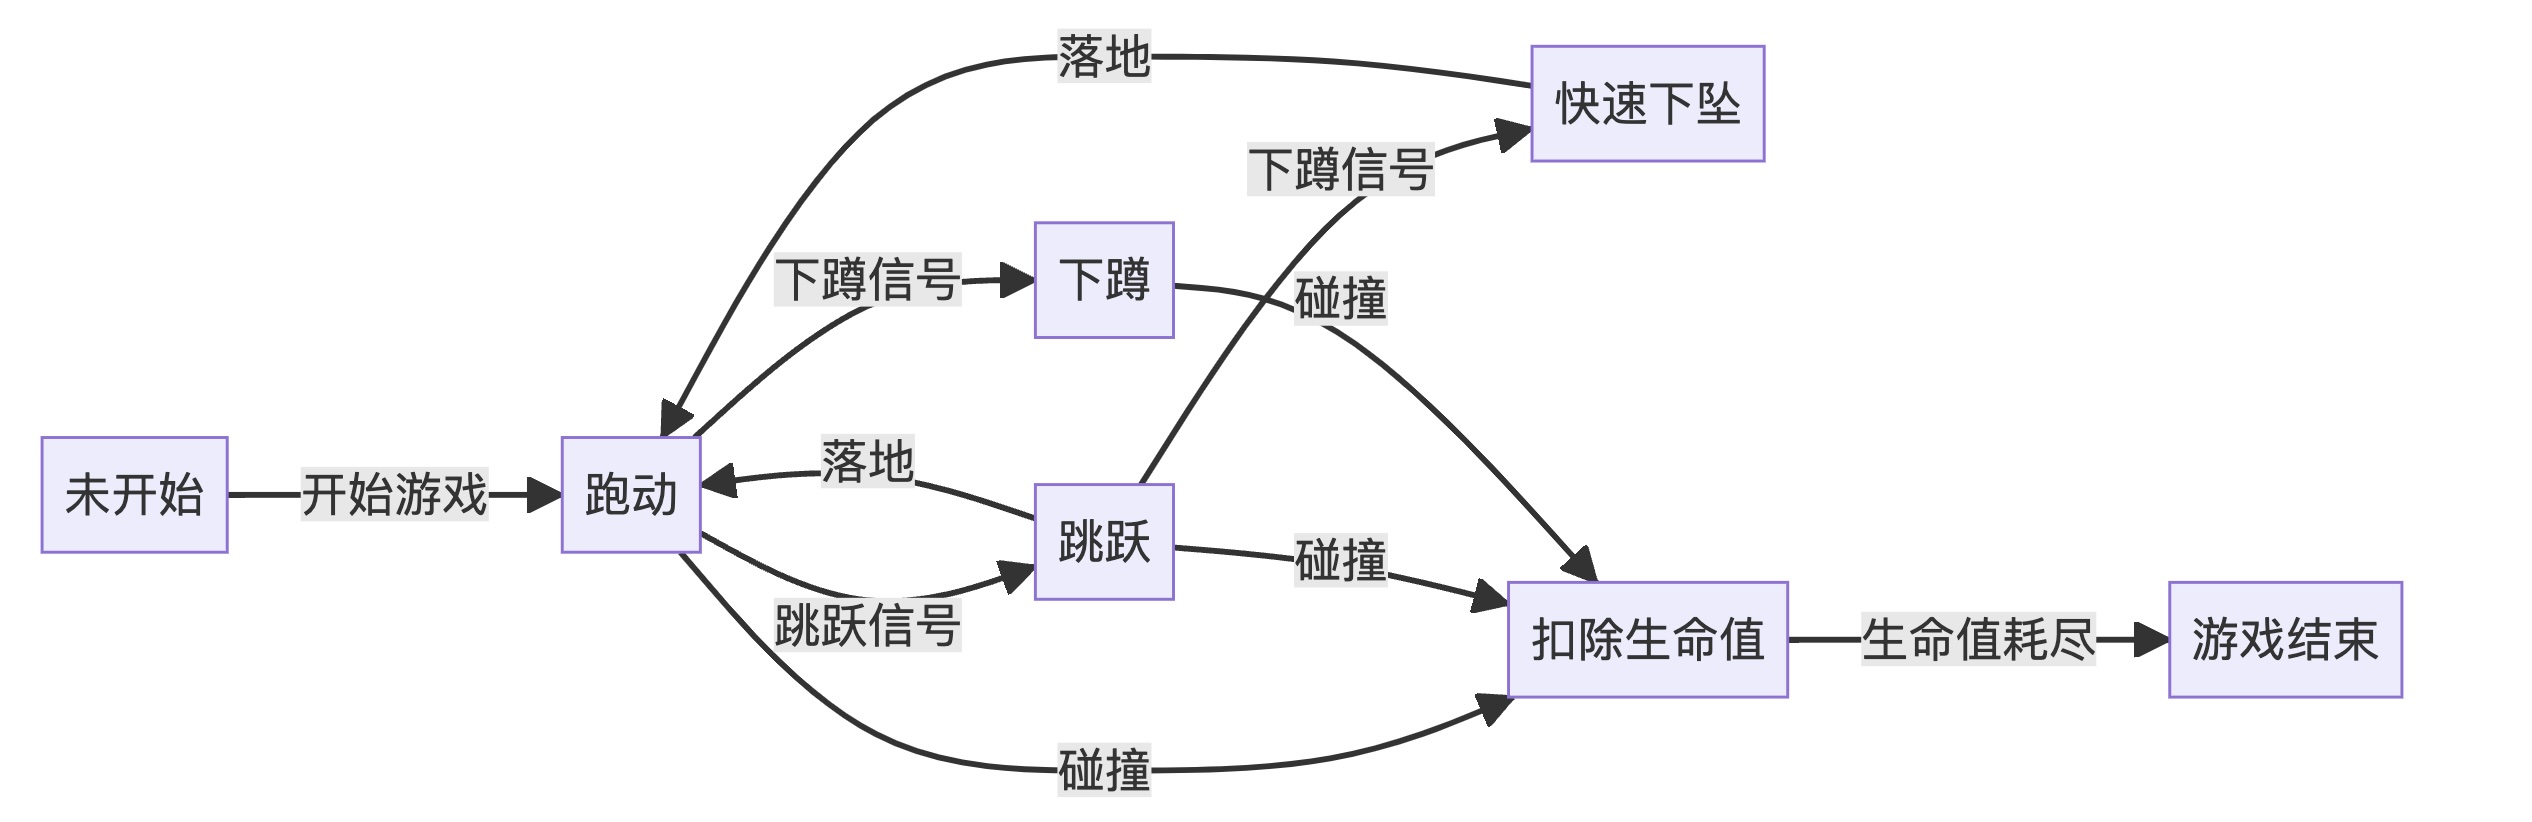
\includegraphics[width=\textwidth]{images/dino-states.jpg}
    \vspace{-16pt}
    \caption{小恐龙状态机}
    \label{dino-states}
\end{figure}

\begin{description}
    \item[未开始] 在这个状态下,小恐龙将会等待游戏开始。接受到跳跃信号时,小恐龙将会进入跑动状态,从而开始运动。
    \item[跑动] 这是小恐龙的一般状态。我们采用了两个材质图像来刻画小恐龙左右脚交替跑动。这个状态可以进行跳跃或者下蹲。 
    \item[跳跃] 在跑动状态下,接收到跳跃信号时,小恐龙将会开始跳跃。根据跳跃信号的时长,跳跃的强度也将不同,即跳跃的高度取决于信号时长。我们也对最低和最高跳跃高度进行了限制,以防运动不稳定或是超出屏幕边界。
    \item[快速下坠] 在跳跃状态下接收到下蹲信号时将进入快速下坠状态,此时小恐龙将会加速下落。玩家可以利用这一特性更加精细地控制自己的运动。
    \item[下蹲] 在跑动状态下,接收到下蹲信号时,小恐龙将蹲下。此时小恐龙的碰撞箱将会变小,可以借此躲过飞行较低的翼龙等障碍。
    \item[扣除生命值] 当碰撞检测模块检测到碰撞时,小恐龙将会进入短暂的免疫状态,在此期间小恐龙的身体会闪烁,且不会再被碰撞检测模块判定为碰撞。这一期间同样也不会有新的障碍生成。
    \item[结束] 当小恐龙的生命值全部扣除完毕时,小恐龙将进入结束状态不再运动。
\end{description}

通过使用状态机,我们使得小恐龙在各种不同状态之间的转换清晰明了,对 SystemVerilog 中任务 (task) 的利用使得我们可以将不同的动作逻辑单独抽出实现,提高了开发效率。

\subsubsection{碰撞检测}

由于我们的游戏元素是通过材质进行显示的,因此我们无法直接通过像素点的坐标来进行碰撞检测。我们采用了碰撞箱 (Collision Box) 的方式进行碰撞检测。

由于直接通过 AABB (Axis-Aligned Border Box) 检测碰撞可能造成误判,考虑到检测准确性与计算时间的权衡,我们将碰撞箱分割成多个子碰撞箱 (\cref{collision})。在检测碰撞时,在小恐龙的任一子碰撞箱与障碍物的任一子碰撞箱发生碰撞时,就判定为碰撞。利用电路执行运算天然的并行特性,我们可以同时进行多个碰撞箱之间的相交检测。

\begin{figure}[H]
    \centering
    
\includegraphics[width=0.2\textwidth]{images/aabb.png}
    
\includegraphics[width=0.2\textwidth]{images/collision-box.png}
    \vspace{-16pt}
    \caption{AABB 与子碰撞箱对比}
    \label{collision}
\end{figure}

\subsubsection{记分板}

在游戏开始后,记分板模块会对速度进行累积来得到当前已经跑过的距离。同时,记分板模块还会记录当前的最高分,以便在游戏结束时进行显示。

最开始时,我们直接记录了跑动距离的值,然后通过将其除以 10 的次幂来得到各个数位进行展示。
然而后来当组合逻辑路径变长时,这导致了时序违约,因为除法运算是比较慢的。
后来,我们也尝试过直接记录各个数位,但这样在需要用到距离的值时,又需要将各个数位重新组合起来,这也会带来额外的开销。
最终,我们发现其实只需要同时维护跑动距离的值和其对应的各个数位,就可以同时满足这两个需求,而且不会带来额外的开销。

\subsubsection{昼夜切换}

为了给小恐龙漫长的旅途带来一些新意,我们添加了昼夜切换机制。每当小恐龙的跑动距离达到一定阈值时,游戏将会进入黑夜模式,此时天空中会出现星星和月亮,所有游戏元素的颜色也将反转。一段时间后,将会切换回白天。

为了使过渡更加平滑,我们采用了渐变的方式进行昼夜切换。具体来说,在距离达到昼夜切换我们会输出 \texttt{night_rate} 信号,这一信号随计时器变动,表明当前的“黑夜程度”。画面输出模块将根据这一信号来计算每一元素的颜色反转程度,从而实现渐变的效果。

另外,这一信号也决定了星星和月亮何时出现。我们手动计算出了背景颜色与星星、月亮颜色恰好一致时的 \texttt{night_rate},从而当 \texttt{night_rate} 达到这一值时,星星和月亮将会自然地出现在天空中。

\section{仿真结果}

由于 ModelSim 不太好用,我们采用 Vivado 进行仿真。

\subsection{传感器数据读取}

\begin{figure}[H]
    \centering
    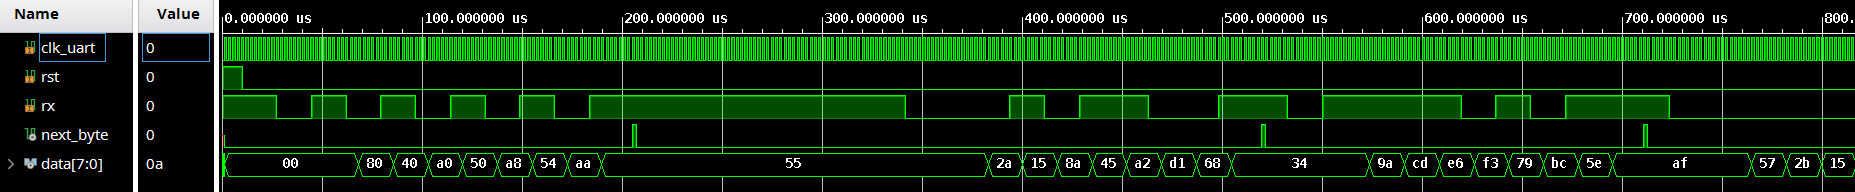
\includegraphics[width=\textwidth]{images/uart-sim-begin.png}
    \vspace{-16pt}
    \caption{\texttt{async_receiver_sim} 仿真结果开头}
\end{figure}

\begin{figure}[H]
    \centering
    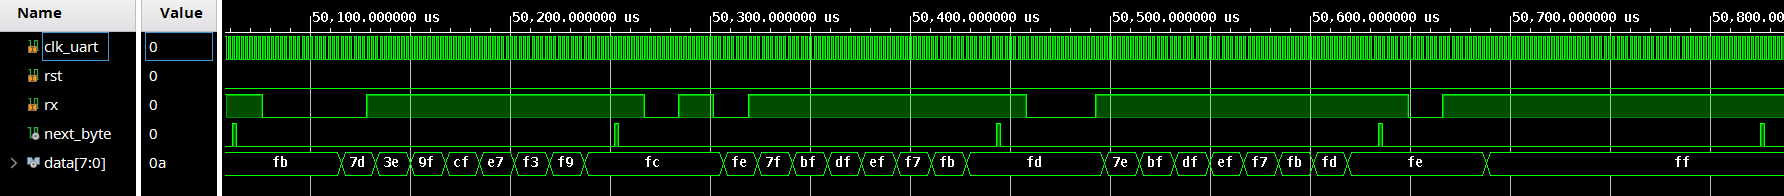
\includegraphics[width=\textwidth]{images/uart-sim-end.png}
    \vspace{-16pt}
    \caption{\texttt{async_receiver_sim} 仿真结果结尾}
\end{figure}

\begin{figure}[H]
    \centering
    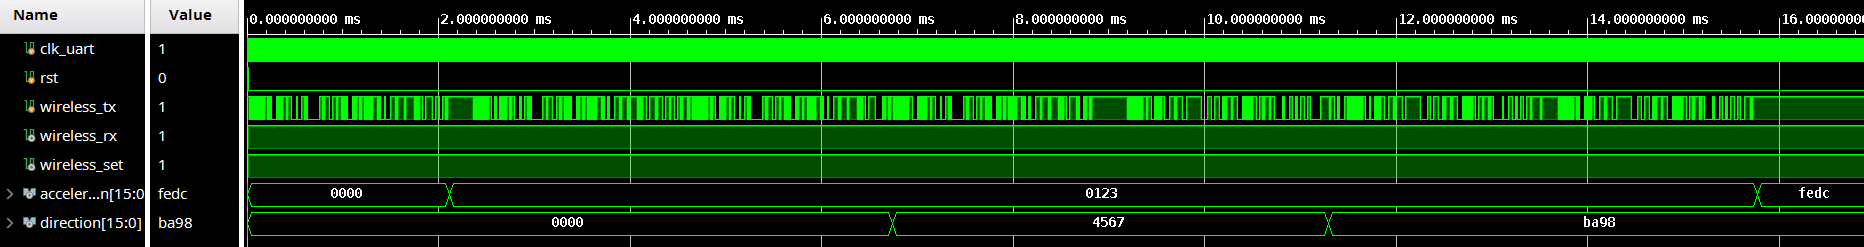
\includegraphics[width=\textwidth]{images/sensor-sim.png}
    \vspace{-16pt}
    \caption{\texttt{sensor_sim} 仿真结果}
\end{figure}

\section{实验演示说明}

\subsection{实验板输入}

两个带去抖按键中,左边的是复位,右边的是跳跃以及开始/重启游戏。四个普通按键中位于右下的是下蹲。16 位拨码开关中最右边的用于控制输入方式,ON 是按键输入,OFF 是传感器输入。

\subsection{传感器使用}

将传感器绑在大腿上,接线的一侧竖直向上,将 USB 转 TTL 模块插入充电宝供电,充电宝放在口袋中或拿在手上。

\section{遇到的问题及解决}

\subsection{外设组装遇到的问题}

一开始我们打算使用面包板进行连线和固定,使用纽扣电池(\SI{6}{\volt} 电池盒 + \SI{3.3}{\volt} 稳压模块)进行供电。

最先遇到的问题是排针没有焊接,导致接触非常不良,几乎完全不可用,焊接后就好了很多。

调试时,先是将无线模块连到电脑上通过无线模块和传感器附带的软件进行调试,这需要使用 USB 转 TTL 模块来与电脑连接。一开始是使用实验板为无线模块供电,就忘了和 USB 转 TTL 模块共地,导致读不到数据。实际上,除了将 USB 转 TTL 模块与实验板共地,更简单的做法是直接通过 USB 转 TTL 模块来为无线模块供电。

使用纽扣电池时,观察到数据传输速率很慢,而且经常过几十秒就完全停止了。经过一系列的排查,最终确定了问题在于纽扣电池的电流太小,无法带动传感器和无线模块。尝试过调整无线模块的工作模式来降低工作电流,情况略有好转但仍然不是很好。于是只能放弃使用纽扣电池供电,改用充电宝供电,之前为了调试购买的 USB 转 TTL 模块刚好可以用来供电。

连到实验板上时还遇到了一个小问题:Pmod 接口的引脚编号和 IO 引脚的序号是不同的,1、2、3、4、7、8、9、10 号引脚分别是 IO0 $\sim$ IO7,一开始没看清导致引脚绑定偏了一位。

这时,外设整体的连接依然不是很稳定,跳几下之后就很容易断开连接,用手稍微按压一下线又会恢复工作。尝试过用透明胶对整体进行固定,有一定的效果,但仍不理想,而且过了几天后可能反而会整体全部松动,需要将胶带拆开才能调整修复。最后改成了所有连线都焊上,连接就非常稳定了。

\subsection{外设数据接收遇到的问题}

一开始是按照 \url{https://www.fpga4fun.com/SerialInterface4.html} 的写法,实现了一个分频,代码会复杂一些,后来才意识到可以通过 PLL 直接生成需要的频率来简化代码并提高准确性。

一开始由于没有理解过采样的作用,而且 fpga4fun 网页上的代码状态机少了一个状态(下载下来的完整代码是正确的),读取每个 bit 的时机(即 \texttt{next_bit} 信号)没有选在 bit 的中点而是选在了边缘,这个错误影响不是很大,但也导致它很难被发现。

\subsection{传感器跳跃检测遇到的问题}

一次典型的跳跃的加速度曲线如\cref{sensor-jump} 所示,一开始先略微上升是在下蹲,后来的一段下降是在加速起跳,后面上升至 0 附近是腾空时接近失重状态,落地时有一个猛烈的下降。

\begin{figure}[ht]
    \centering
    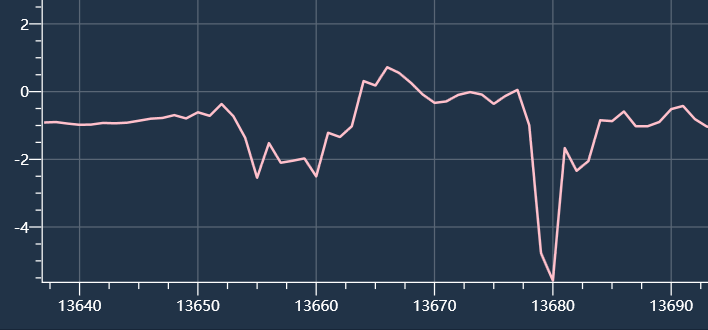
\includegraphics[width=0.8\textwidth]{images/sensor-jump.png}
    \caption{跳跃时传感器检测到的加速度曲线}
    \label{sensor-jump}
\end{figure}

最终采用的阈值判断本质上是在检测腾空的这一段,这导致检测到的时机略晚于起跳,会让玩家感到一定的延迟,影响游戏体验,所以我们尝试了多种方法来试图优化跳跃检测的灵敏性、准确性和即时性。但最后这些方法都没有取得更好的效果,只能退而求其次,通过给玩家多条生命来缓解游戏难度过高带来的问题。

\subsubsection{对加速度积分得到速度}

仅检测加速度是不太准确的,如果能检测速度就会好很多。但是简单地积分会产生严重的累积误差,传感器的时间粒度也不够细,而且传感器检测到的不是实际运动的加速度,而是带 $g$ 的加速度,为了得到实际运动的加速度就需要得到 $g$ 的值,而 $g$ 的误差又会带来更严重的累积误差。所以我们最终放弃了这一方案。

\subsubsection{检测全方位总加速度而非竖直方向加速度}

因为本质上是在检测腾空的这一段,而腾空时近似处于失重状态,其实可以不止检测竖直方向加速度,而是检测总加速度,总加速度(的绝对值)足够小就可以视为是腾空,这样的话可以一定程度上避免下蹲之类的动作被误识别为腾空,从而允许设置更宽松的阈值。这个思路应该是没有太大问题的,但实际测试时发现效果和之前差不多甚至略差。一个可能的解释:从\cref{sensor-jump} 中可以看出,腾空最开始时有一段加速度远超 $0$,判断竖直方向加速度时只需判断加速度大于一个负数,判断总加速度时则是判断加速度绝对值小于一个数,这会导致过大的加速度被漏判。

\subsubsection{检测起跳而非腾空}

检测腾空不可避免地会有一定的延迟,但检测起跳的主要问题在于,起跳和落地的加速度曲线是类似的,需要想办法进行区分。

起跳的持续时间往往比落地长,但持续时间会因玩家动作而有较大的变化,如果检测起跳的持续时间,一方面可能造成误判、漏判,另一方面也会导致检测不及时。

还有一个思路是在检测到腾空后的短时间内禁用跳跃检测,但这样在理论上就会有连跳被漏判的风险,实际测试时效果也非常不好。

\subsection{画面输出遇到的问题}

在存 sprite 图时,一开始使用的是 \href{https://github.com/thu-cs-lab/MifConverter}{MifConverter},得到的 MIF 文件字宽不对,而 MifConverter 只支持 8 的倍数的字宽,所以自己写了一个脚本来进行转换。

为了避免出现时序问题,需要降低元素绘制使用的时钟频率,但为了在一帧内完成显存的写入,至少需要 $1280 \times 300 \times 60 \times (1+\alpha)$ 的时钟频率,其中 $\alpha$ 表示画面上所有元素的 bounding rectangle 大小之和占画面总大小的比例。最终我们选择了使用 \SI{33.33}{\mega\hertz} 的时钟,这允许大约 \SI{40}{\percent} 的画面元素占比。

在信号跨时钟域时如果不处理好也会出现时序问题,最简单且可靠的处理方式是使用一个写入时钟和读取时钟不同的只存 1 bit 数据的 RAM IP 核。

除了降低时钟频率,也需要避免使用组合逻辑进行输出,对每个输出信号加上 buffer 即可。

\subsection{运算溢出 \& 符号问题}

由于对 SystemVerilog 的数据类型体系不够熟悉,在类型不同的整数混合运算时,碰上了不少各种各样的问题,例如障碍物间隔计算溢出导致多个障碍重叠地生成,运算的符号不正确导致元素位置不对等等。

在这里,我简单总结一下 SystemVerilog 中整数的类型系统以及对不同类型的整数进行混合运算时的规则:
\begin{itemize}
    \item 逻辑向量默认是无符号类型;
    \item 可以通过 \texttt{signed} 来声明有符号逻辑向量,例如 \texttt{logic signed [15:0]};
    \item 定宽整数类型(如 \texttt{integer})默认是有符号类型;
    \item 参数 (\texttt{parameter}) 的默认类型是 \texttt{integer},因此是有符号的;
    \item 纯数字字面量(不含进制)如 \texttt{233}, \texttt{-42} 属于 \texttt{integer} 类型,因此是有符号的;
    \item 含有进制信息的字面量如 \texttt{'h3c}, \texttt{4'b1010} 属于逻辑向量类型,因此是无符号的;即使不含位数信息也是如此,此时是 32 位无符号逻辑向量;
    \item 含有进制信息的字面量可以通过 \texttt{s} 来标记为有符号逻辑向量,例如 \texttt{'sh3c};
    \item 不同类型的整数混合运算时,首先决定结果是否有符号:当且仅当所有运算数都有符号时,结果有符号,否则结果为无符号数;其次根据运算数中最长的位宽(以及结果的位宽,如果已知)来扩展运算数并进行运算。
\end{itemize}

另外需要注意的是,位宽相同时,有符号的变量的绝对值的范围会变小约一半,在决定变量位宽时需要考虑这一点。

\subsection{时序问题}

时序问题导致了各种各样的奇怪现象:
\begin{itemize}
    \item 时序违约时,绘制模块来不及绘制完所有场景元素 VGA 就触发了更新,导致画面出现拖影等;通过优化时序可以解决;
    \item 游戏逻辑模块采用内部计时器时,由于计时的累积误差,有可能导致逻辑模块与绘制模块同时运行,此时绘制出的元素状态不正确;通过让绘制模块通知逻辑模块更新时机解决此问题;
    \item 设置了一级延迟的除法器 IP 实际上在状态机中需要两个状态进行等待,因为给出除法器的输入也需要花费一个状态,在设计状态转移时需要考虑这一点。
\end{itemize}

\subsection{组合逻辑}

组合逻辑的输出有时并不稳定,很容易导致各种奇怪现象:
\begin{itemize}
    \item 当 VGA 输出采用组合逻辑时,若输出不稳定则整个画面会黑屏,通过将输出信号加上 buffer 可以解决;
    \item 曾经观察到按下复位按钮后,记分板有时会出现其中一位为 1 的怪现象,经过检查发现是直接将复位按钮接入到了 \texttt{rst} 信号,若按下按钮的时机恰好落在时钟上升沿的设置时间内则可能导致各种不可预测的问题;通过将外部输入信号加上 buffer 可以解决;
    \item 某些模块采用组合逻辑进行计算,直接将输出信号接入到其他模块的输入信号上可能会导致不稳定和元素的抖动,通过将输出信号加上 buffer 可以解决。
\end{itemize}

可以发现有许多问题都能通过增加 buffer 解决。

\end{document}
